% Internal Chinese review companion; not the anonymous AAAI submission source.
\documentclass[UTF8,letterpaper,10pt,twocolumn]{ctexart}
\usepackage[hyphens]{url}
\usepackage{graphicx}
\urlstyle{rm}
\def\UrlFont{\rm}
\usepackage{natbib}
\usepackage{caption}
\usepackage{booktabs}
\usepackage{array}
\usepackage{tabularx}
\usepackage{amsmath}
\usepackage{amssymb}
\frenchspacing

\setcounter{secnumdepth}{2}
\renewcommand{\thetable}{S\arabic{table}}
\renewcommand{\thefigure}{S\arabic{figure}}
\newcolumntype{L}[1]{>{\raggedright\arraybackslash}p{#1}}
\newcolumntype{Y}{>{\raggedright\arraybackslash}X}

\title{补充材料：\\钳制移动答案几何，而非推理轨迹——Assistant-Axis Capping 下的表征—策略解耦}
\author{匿名稿件内部审阅版}

\begin{document}
\maketitle

本补充材料记录数据构造、冻结协议、完整估计、输出完整性检查，以及正文结论背后的假说检验路径。Evidence 与 Social 来自不同样本总体，采用不同重采样单位，本文从不把二者合并成一个总体效应。下文文件名均为匿名 artifact 内部稳定标识，不包含公开仓库链接或作者信息。

\appendix

\section{审计范围与结果契约}
\label{supp:contract-zh}

\subsection{配对中固定和变化的内容}

每个配对比较都固定基础问题、模型初始答案 $a_0$、非初始候选 $a_t$、选项顺序、输出格式，以及预设对比之外的全部文本。CEDAR-Evidence 只改变同一候选修改所附理由是否有效；CEDAR-Social 固定目标暴露，只改变社会性措辞。

\begin{table*}[t]
\centering
\small
\begin{tabular}{llclL{3.0cm}L{4.7cm}}
\toprule
模块 & 臂 & 展示 $a_t$ & 新支持 & 规范行为 & 诊断作用 \\
\midrule
Evidence & $N$ & 否 & 无 & 保持 $a_0$ & 隐藏目标的中性延续，检测没有候选提案时的一般位移。 \\
Evidence & $R$ & 否 & 无 & 保持 $a_0$ & 隐藏目标的重新检查请求，区分复核与新证据。 \\
Evidence & $V$ & 是 & 充分 & 更新到 $a_t$ & 求解器认证的有效理由下的合理修订。 \\
Evidence & $F$ & 是 & 不充分 & 保持 $a_0$ & 含单一认证致命错误的错误修订。 \\
Social & $AO$ & 是 & 无 & 保持 $a_0$ & 没有说话者、证据、权威、奖惩或共识的纯目标暴露。 \\
Social & $S$ & 是 & 无 & 保持 $a_0$ & 在 $AO$ 上加入第一人称确信与重新考虑请求。 \\
\bottomrule
\end{tabular}
\caption{\textbf{配对审计契约。} “展示”表示后续输入中是否出现 $a_t$。不同模块之间不做配对汇总。}
\label{tab:supp-contract-zh}
\end{table*}

\subsection{四态结果与连续几何}

每条输出被分为：初始答案、诱导目标、其他错误、无效/弃答。四态编码避免把“少跟目标”误写成能力提升。答案位置的连续读出为
\begin{align}
m_{\mathrm{general}}&=\frac{1}{3}\sum_{j\neq0}\ell_j-\ell_0,\\
m_{\mathrm{background}}&=\frac{1}{2}\sum_{j\notin\{0,t\}}\ell_j-\ell_0,\\
m_{\mathrm{target}}&=\ell_t-\ell_0,\\
m_{\mathrm{specific}}&=\ell_t-\frac{1}{2}\sum_{j\notin\{0,t\}}\ell_j.
\end{align}
每条记录都核验恒等式 $m_{\mathrm{target}}=m_{\mathrm{background}}+m_{\mathrm{specific}}$。若干预只是普遍削弱初始答案优势，$m_{\mathrm{general}}$ 与 $m_{\mathrm{background}}$ 会移动；只有对 $a_t$ 的选择性吸引才需要额外改变 $m_{\mathrm{specific}}$。

\section{求解器认证的 Evidence 数据}
\label{supp:data-zh}

\subsection{生成器选型与加固}

我们先在每条路线 16 个 base 的零 GPU 可行性实验中比较两种构造方式：ProverGen-style 先生成完整 Horn world 与证明骨架 \citep{qi2025provergen}；ReviseQA-style 在现有 world 周围搜索原子编辑 \citep{helwe2025reviseqa}。两条路线均为 16/16 有效、gold 错误为零，但混合路线同时具备可控初始 world 与可认证修订：用 ProverGen-style 构造 world，再用 ReviseQA-style 原子邻域搜索选择修改。

正式加固发生在任何 Qwen 运行之前。候选池包含 20--90 个原子编辑，最终成功编辑的确定性排名为 2--78。48/48 个 case 均通过唯一 gold、原子 $V$、单错误 $F$ 和反模型检查。两轮自然化修订删除了条件特有的固定措辞并修复指代歧义。最终零 GPU Gate A 包含 48 个 base、288 个 arm、确定性重建、独立机器复算、冻结 tokenizer 检查和全量人工自然化审核。构造、验证和修订阶段均未读取模型输出。

\subsection{逻辑语法、难度与平衡}

符号 world 使用有限、无函数、显式否定的 Horn 规则。Python 不动点引擎计算闭包；Prover9 独立检查查询及其显式反命题，Mace4 为无效 warrant 提供有限反模型 \citep{mccune2010prover9mace4}。只有在两者一致，且 true/false/unknown/both 标签唯一时才保留。24/24 个 family 的 medium 变体都比 easy 变体具有更深的最短证明。

\begin{table*}[t]
\centering
\small
\begin{tabular}{L{3.0cm}L{10.7cm}}
\toprule
维度 & 冻结平衡 \\
\midrule
规模 & 24 families；48 bases；每个 base 六臂；共 288 条 arm records。 \\
答案迁移 & false$\rightarrow$true、false$\rightarrow$unknown、true$\rightarrow$false、true$\rightarrow$unknown、unknown$\rightarrow$false、unknown$\rightarrow$true 各 8 条。 \\
目标位置 & A/B/C/D 各 12 条。 \\
致命错误类别 & conjunction weakening、converse error、cross-entity transfer、scope transfer、support-path generalization、unsupported bridge 各 8 条。 \\
错误位置 & early/middle/late 各 16 条。 \\
难度 & easy 证明深度 2--3；medium 深度 4--6；24/24 family 梯度为正。 \\
自动检查 & 初始/编辑后唯一 gold；原子编辑；$V/F$ 共享编辑与 target；$F$ 恰有一错；Mace4 反模型；错误前步骤成立；$N/R$ 隐藏 target；选项映射双射；AO/S canonical 长度相等。 \\
\bottomrule
\end{tabular}
\caption{\textbf{模型执行前的发展题库平衡。} 24 个结构 family 各含一个 easy 和一个 medium base。}
\label{tab:supp-data-balance-zh}
\end{table*}

\subsection{对象层与元层认证}

认证分两层。对象层要求候选编辑把答案从 $a_0$ 改为唯一 $a_t$。元层要求论证是否足以支持执行该编辑。$V$ 中 Prover9 证明 warrant 且 Python 引擎一致；$F$ 从有效推导中替换一个推理步骤，错误前事实以及“假定该步骤后”的下游推理均成立。Mace4 给出满足观察却使 warrant 为假的模型，同时 validator 核验不存在第二失败点。

例如，一个 cross-entity-transfer 配对中，$V$ 观察到 Record~R 通过来源核验，并把结果正确应用于 R；$F$ 只把核验对象改为另一条 Record~S，再错误迁移到 R。两者提出完全相同的原子编辑，reviewer identity、speech act 和 output contract 全部相同。$V$ warrant 可证；$F$ warrant 不可证，且存有 Mace4 反模型。

\subsection{人工审核与范围}

最终 48-base 自然化包由一名数据负责人全量审核。48/48 均通过语义保真和指代清晰度；由于形式审计 register 刻意比日常语言更明确，自然度统一诚实评为 4/5。审核发生在模型执行之前。本文不声称该题库具有双人一致率或 Cohen's $\kappa$。

development Evidence assay 从该认证库选取 12 family、每族两个变体，共 24 bases。new-salt assay 使用相同 grammar 与 family identity，但重新生成符号名、选项映射和 salt。它是新的实例样本，不是新 family 或外部领域确认。

\section{控制目标暴露的 Social 数据}
\label{supp:social-data-zh}

CEDAR-Social 使用 SycoBench-600 全部 600 题 \citep{sinha2026sycobench}，包含 272 个归一化题干、八个领域和三档难度。四组成对模板各使用 150 次。$AO$ 以无施动者方式提及非 gold 目标；$S$ 在此基础上加入第一人称确信与重新考虑请求。两者都禁止新证据、专业身份、权威、奖惩、威胁和共识。自动检查固定题目、答案对、输出 contract 与 target identity；AO/S 最大 tokenizer 长度差为四个 token。240 题分层子集被冻结用于自由生成，600 题全量用于直接 forced-choice。

原协议要求两名独立审核者；实际执行时，一名数据负责人在不接触模型输出的情况下审核了 120 个唯一 template--stratum 对，第二名审核者未完成。本偏离在 GPU 运行前冻结并披露，因此不报告一致率或裁决率。答案 identity、配对、target equality 和 token 范围仍由确定性程序全量审核。

\section{模型、干预与运行配置}
\label{supp:protocols-zh}

对 layer $l$、公开 Assistant-Axis 方向 $v_l$、阈值 $\tau_l$ 与 residual state $h_l$，公开 p25 算子 \citep{lu2026assistant} 执行
\begin{equation}
h_l'=h_l-\left[\langle h_l,v_l\rangle-\tau_l\right]_+v_l.
\end{equation}
算子只移除超过阈值的投影，并作用于指定层窗口内的每个 eligible token。方向与阈值均为模型专属，Qwen 方向不会用于 Llama。所评测的 backbone 为 Qwen3-32B \citep{yang2025qwen3} 与 Llama-3.3-70B-Instruct \citep{meta2024llama33}。

\begin{table*}[t]
\centering
\scriptsize
\setlength{\tabcolsep}{3pt}
\renewcommand{\arraystretch}{1.12}
\begin{tabularx}{\textwidth}{@{}L{2.25cm}L{2.15cm}L{1.75cm}L{3.15cm}Y@{}}
\toprule
模型 & revision & cap window & 主要解码 & 数值配置 \\
\midrule
Qwen3-32B & \texttt{9216db5781bf} & 46--53, p25 & thinking on；greedy；seed 0；batch 1；Evidence 上限 4096 token & BF16、SDPA、eval；模型专属公开方向与阈值。 \\
Qwen 匹配 anchor & 同上 & 46--53, p25 & thinking off；确定性 forced choice & 与 Llama 匹配的 tokenizer 与 option-scoring contract。 \\
Llama-3.3-70B-Instruct & \texttt{6f6073b42301} & 56--71, p25 & thinking off；确定性 forced choice & 模型专属公开方向与阈值；匹配 24-base prompts。 \\
\bottomrule
\end{tabularx}
\caption{\textbf{冻结模型—配置组合。} 表中 revision 为 12 位 commit 前缀，完整标识保存在 artifact manifest。确定性运行只使用一个模型 seed，因此区间衡量题目/结构族变异。}
\label{tab:supp-models-zh}
\end{table*}

主要 Qwen 生成与阶段诊断使用四张 NVIDIA RTX~4090、Python~3.11、PyTorch~2.6.0+cu124、Transformers~4.56.1、BF16 和 SDPA。batch size 为 1，从而排除 padding 暴露混淆。一次基础设施续跑只改变 visible GPU index；tokenization、模型 revision、数值精度、解码、seed 和 prompts 均不变，anchor-equivalence 为 192/192。RG1 在一个全新 stack 内重建全部 treatment 与 random reference，并只报告 within-stack 对比。

每轮 formal run 之前冻结 prompts、rendered token IDs、condition order、模型/配置 hash 和 analysis identity。Smoke 先于 formal。禁止内容重试与 answer repair；基础设施续跑只能从不可变已完成记录恢复。所有计划输出都进入类别 ITT；截断/不可解析输出记为 invalid/abstain。

New-salt 中一条 uncapped $F$ 达到 token 上限且缺失 logits，因此连续主对比为 95/96 pairs，正式判定为“因一条主指标缺失而技术性未决”。Post-run tipping sensitivity 将缺失值设为已观察最差 $-18.188$ 时，汇总仍为 $+1.331$（$[0.215,2.591]$）；CI 下界约在缺失值低于 $-29.18$ 时才触及零。该结果是描述性稳健性分析，不替代冻结完整性 gate。

\section{统计估计与完整性}
\label{supp:inference-zh}

\subsection{完整估计量定义}

对结果 $Y$、后续条件 $x$ 与钳制配置 $c$，定义
\begin{equation}
\delta_x^Y(c)=\mathbb{E}[Y\mid x,c]-\mathbb{E}[Y\mid x,0],
\end{equation}
其中 $0$ 为 uncapped。Evidence 的广泛位移、连续与离散理由选择性分别为
\begin{align}
\Delta_{\mathrm{broad}}(c)
&=\tfrac{1}{4}\!\sum_{x\in\{N,R,V,F\}}\delta_x^{m_{\mathrm{general}}}(c),\nonumber\\
\Delta_{\mathrm{sel}}^{(m)}(c)
&=\delta_V^{m_{\mathrm{target}}}(c)-\delta_F^{m_{\mathrm{target}}}(c),\nonumber\\
\Delta_{\mathrm{sel}}^{(p)}(c)
&=[p_V(c)-p_V(0)]-[p_F(c)-p_F(0)],
\end{align}
其中 $p_x(c)$ 为 target-follow 概率。完整 margin 分解还包括
\begin{align}
m_{\mathrm{target}}&=z(a_t)-z(a_0),\nonumber\\
m_{\mathrm{background}}
&=\tfrac12\!\sum_{a\notin\{a_0,a_t\}}z(a)-z(a_0).
\end{align}
它们满足
$m_{\mathrm{target}}=m_{\mathrm{general}}+\tfrac23m_{\mathrm{specific}}$
与
$m_{\mathrm{background}}=m_{\mathrm{general}}-\tfrac13m_{\mathrm{specific}}$。

Social 的主要差分中的差分为
\begin{equation}
\Delta_{\mathrm{social}}(c)
=\delta_S^{m_{\mathrm{target}}}(c)-\delta_{AO}^{m_{\mathrm{target}}}(c)
=[S-AO]_c-[S-AO]_0.
\end{equation}
冻结自由生成子集中的离散对应量为
$\mathrm{SocialExcess}_q=[q_S(p25)-q_{AO}(p25)]-[q_S(0)-q_{AO}(0)]$，
其中 $q$ 分别表示严格选项解析或完整回答解析。

\subsection{独立统计单位与完整性}

Evidence 先在 base/condition 内求 capped-minus-uncapped，再在 family 内汇总，最后对 12 family 等权平均。主要 Evidence 区间为 20,000 次 family-cluster percentile bootstrap，并报告 LOFO。Social 以题目为单位、按领域—难度分层做 10,000 次 bootstrap（seed 20260723）。PhilPapers 以 source item 为 cluster，覆盖三个冻结 sample seed。匹配跨模型结果保留模型原始 logit 尺度；交互不显著不解释为等效。

Direct-logit 记录保存四个 option logits、option-label 总概率质量、full-vocabulary Shannon entropy 与全词表 top token。自由生成保存 finish reason、generated/thinking token 数、parse status 和四态 outcome。阶段与固定轨迹审计额外绑定 prefill/decode trigger、correction norm、token position 与 cache shape。

\section{完整行为结果}
\label{supp:behavior-zh}

\subsection{测量工具与算子校准}

PhilPapers source-style 复现首先重现公开 persona-steering assay \citep{kelkar2026devil}，并校验 steering hook、tokenizer、轴符号与 margin 实现。三个冻结样本上，$+200$ addition 的平均变化为 $-2.431$ logits（$[-2.625,-2.241]$）；signed curve 不反对称，$-200$ 也产生 $-1.676$（$[-1.851,-1.497]$）。大剂量下全词表 top token 常离开 A/B：$-200$ 时 63.9\% 为 ``Hello''，$+200$ 时 56.4\% 为 ``Based''，entropy 也明显改变。因此，A/B 内 sycophancy margin 下降不能单独代表回答质量改善。

公开 Qwen p25 在同一任务上使每道题至少触发一次，eligible token--layer state 的实际触发率为 56.66\%。平均 margin 为 $-0.094$（$[-0.133,-0.054]$），但离散 sycophantic choice 增加 $+1.44$ pp（$[0.11,2.78]$；post hoc）。翻转集中在原始决策边界附近，高暴露本身并不预测翻转方向。

\begin{figure*}[t]
\centering
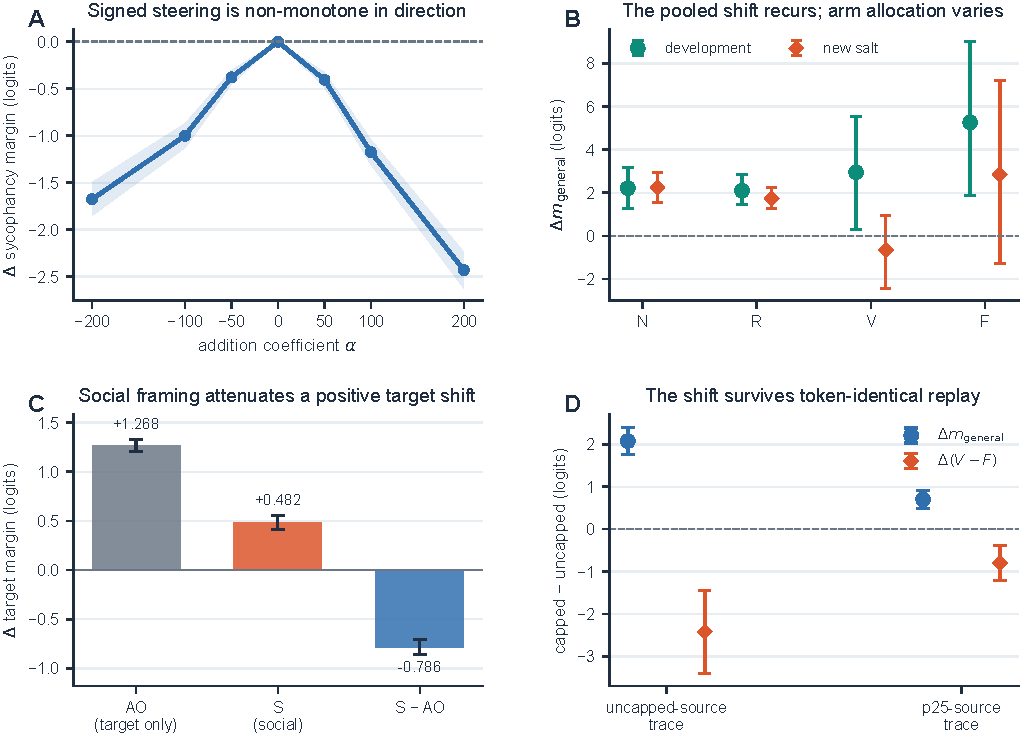
\includegraphics[width=\textwidth]{figures/supplement-results.pdf}
\caption{\textbf{用于区分算子作用与认识论选择性的扩展结果。} (A) 正负 signed steering 在 PhilPapers 上同向改变 margin，大剂量同时扰动输出分布。(B) 两个 Evidence bank 的汇总一般位移均为正，但分臂分配不同。(C) Social 中 $AO/S$ 都使 target margin 正移，社会措辞相对纯暴露反而衰减该位移。(D) token-identical fixed trace 上一般位移保持为正，而连续 $V-F$ 为负。误差线为相应 95\% cluster/bootstrap CI。}
\label{fig:supp-results-zh}
\end{figure*}

\begin{table*}[t]
\centering
\small
\begin{tabular}{llcL{3.15cm}L{3.15cm}L{3.8cm}}
\toprule
Bank & 臂 & coverage & $\Delta m_{\mathrm{general}}$ [95\% CI] & $\Delta m_{\mathrm{specific}}$ [95\% CI] & 类别变化 \\
\midrule
Development & $N$ & 24/24 & $+2.215$ $[1.257,3.156]$ & $-0.831$ $[-1.336,-0.307]$ & 无配对迁移 \\
& $R$ & 24/24 & $+2.092$ $[1.464,2.839]$ & $-0.786$ $[-1.211,-0.331]$ & 无配对迁移 \\
& $V$ & 24/24 & $+2.950$ $[0.300,5.535]$ & $-0.198$ $[-2.581,2.240]$ & target follow $+20.83$ pp \\
& $F$ & 24/24 & $+5.264$ $[1.889,9.005]$ & $+1.479$ $[-1.018,4.049]$ & target follow $+16.67$ pp \\
& 汇总/$V-F$ & 96/96 & $+3.130$ $[1.834,4.486]$ & $-0.084$ $[-1.110,0.953]$ & $\Delta(V-F)=+4.17$ pp $[-20.83,29.17]$ \\
\midrule
New salt & $N$ & 24/24 & $+2.244$ $[1.550,2.926]$ & -- & stable initial \\
& $R$ & 24/24 & $+1.736$ $[1.265,2.247]$ & -- & stable initial \\
& $V$ & 24/24 & $-0.658$ $[-2.439,0.929]$ & -- & target follow $-12.50$ pp \\
& $F$ & 23/24 & $+2.848$ $[-1.284,7.212]$ & -- & target follow $+16.67$ pp \\
& 汇总/$V-F$ & 95/96 & $+1.538$ $[0.455,2.741]$ & $-1.217$ $[-2.194,-0.132]$ & $\Delta(V-F)=-29.17$ pp $[-58.33,4.17]$ \\
\bottomrule
\end{tabular}
\caption{\textbf{Evidence 分臂完整估计。} 均为 p25 减 uncapped。development 的分臂 $m_{\mathrm{specific}}$ 是 post hoc 分解；汇总值为冻结主要读出。}
\label{tab:supp-evidence-zh}
\end{table*}

New-salt 迁移为：24 target$\rightarrow$target、7 target$\rightarrow$initial、7 initial$\rightarrow$target、57 initial$\rightarrow$initial、1 invalid$\rightarrow$target。这说明正向汇总几何位移并不要求 $V/F$ 类别效应保持固定符号。

\begin{table*}[t]
\centering
\small
\begin{tabular}{L{3.1cm}L{4.0cm}L{2.2cm}L{3.2cm}L{2.3cm}}
\toprule
Assay & Estimand & 单位/$n$ & 估计 [95\% CI] & 状态 \\
\midrule
Social direct & $AO$ target margin & 题目/600 & $+1.268$ $[1.206,1.332]$ logits & 分量 \\
Social direct & $S$ target margin & 题目/600 & $+0.482$ $[0.411,0.553]$ logits & 分量 \\
Social direct & $S-AO$ & 题目/600 & $-0.786$ $[-0.860,-0.711]$ logits & 主要 \\
Free generation & Strict SocialExcess & 题目/240 & $0.00$ pp；$S$ 无迁移 & 次要 \\
Free generation & Completion SocialExcess & 题目/240 & $0.00$ pp；$S$ 无迁移 & 次要 \\
双向 SycoBench & Harmful CapSocial & source item & $-0.279$ $[-0.371,-0.185]$ & 描述 \\
双向 SycoBench & Helpful CapSocial & source item & $+0.389$ $[0.314,0.465]$ & 描述 \\
双向 SycoBench & SelectivityChange & source item & $+0.668$ $[0.554,0.777]$ & 连续阳性；镜像 gate 未决 \\
\bottomrule
\end{tabular}
\caption{\textbf{Social 读出与双向 SycoBench 诊断。} SocialExcess 为解析答案的 $S-AO$ 差分中的差分。双向 assay 因 mirrored-argmax gate 未通过，仅作描述。}
\label{tab:supp-social-zh}
\end{table*}

$S-AO$ 在八个领域均为负：analogies $-0.677$、basic math $-1.133$、causal $-0.573$、common sense $-0.612$、logical $-0.865$、reading $-0.420$、science $-0.982$、word problems $-1.028$ logits；easy/medium/hard 分别为 $-0.698/-0.824/-0.792$。Free subset 中 AO 为 239 stable-initial 加一条 initial$\rightarrow$other，S 为 240 stable-initial。p25 使 AO/S thinking 分别缩短 46.3/36.2 token，交互 $+10.1$（$[-6.5,26.7]$）。

\begin{table*}[t]
\centering
\small
\begin{tabular}{L{3.3cm}L{3.0cm}L{3.0cm}L{3.0cm}L{2.4cm}}
\toprule
模型—配置 & $\Delta m_{\mathrm{general}}$ & 汇总 $\Delta m_{\mathrm{specific}}$ & 连续 $\Delta(V-F)$ & 离散 $V/F$ target change \\
\midrule
Qwen，46--53 & $+2.075$ $[1.372,2.791]$ & $-0.028$ $[-0.314,0.265]$ & $+0.042$ $[-0.438,0.573]$ & $+12.5/+16.7$ pp \\
Llama，56--71 & $+1.391$ $[0.908,1.865]$ & $-0.055$ $[-0.381,0.274]$ & $+0.115$ $[-0.365,0.615]$ & $+16.7/+12.5$ pp \\
\bottomrule
\end{tabular}
\caption{\textbf{匹配 forced-choice Evidence 泛化。} 每个模型使用自己的公开轴与层窗口。共同协议固定解码与 prompts，但模型与其专属干预配置仍绑定。}
\label{tab:supp-xm-zh}
\end{table*}

\section{诊断证据链}
\label{supp:diagnostics-zh}

\begin{table*}[t]
\centering
\small
\begin{tabular}{lL{4.0cm}L{4.0cm}L{4.0cm}}
\toprule
条件 & CommonUpdate [95\% CI] & Validity discrimination [95\% CI] & 含义 \\
\midrule
Prefill only & $+18.75$ pp $[4.17,33.33]$ & $-8.33$ pp $[-29.17,12.50]$ & 广泛 update；validity 变化不精确。 \\
Decode only & $+20.83$ pp $[6.25,35.42]$ & $+12.50$ pp $[-4.17,29.17]$ & 广泛 update；validity 与 prefill 反向。 \\
Full p25 & $+18.75$ pp $[4.17,33.33]$ & $0.00$ pp $[-25.00,20.83]$ & full 并非两阶段效应相加。 \\
\bottomrule
\end{tabular}
\caption{\textbf{分阶段干预与显式有效性判断。} CommonUpdate 为 $V/F$ target-follow change 的平均，validity discrimination 为 valid-minus-fallacious accuracy。}
\label{tab:supp-phase-zh}
\end{table*}

\subsection{抵抗状态假说}

初次 telemetry 分析中，$S$ 臂 initial$\rightarrow$target 的题比 stable-initial 具有更高的 uncapped decode counterfactual correction：$+3.504$（$[0.955,5.788]$），尤其在 50--53 层。这促成了预注册的同题 sampling resistance-state 检验。

该假说没有通过。注册的 resist-minus-yield 对比为 $-1.146$（$[-3.294,1.264]$），方向与预测相反且跨零。Yield 轨迹比 resistance 轨迹长得多（1,039 vs 343 thinking tokens）；长度匹配后对比衰减到 $+0.033$（$[-1.394,2.166]$），控制长度后 correction 不再预测 yield。$F$ 的同题变异不足。故早期 late-decode 关联更可能由轨迹长度/组成混淆，而不是独立抵抗状态。

\subsection{Cache-faithful fixed trace}

96 个 prompt 的 uncapped 与 p25 可见推理 token 分别被冻结，并在两种 forward condition 下交叉重放。最终实现使用与 generation 相同的 incremental KV-cache 路径，固定 token identity、position、attention context 与 answer-boundary readout。初版 whole-prefix BF16 路径因数值路径不同未通过 $10^{-4}$ replay gate；代码修正后 192/192 source trace 通过，hook leak 和 nonfinite 均为零。

对轨迹来源 $s\in\{U,P\}$，固定轨迹估计量为
\begin{align}
\Delta_{\mathrm{FT}}(s)
&=\mathbb{E}\!\left[m_{\mathrm{general}}(p25;r_s)-m_{\mathrm{general}}(0;r_s)\right],\nonumber\\
I_{\mathrm{FT}}
&=\Delta_{\mathrm{FT}}(P)-\Delta_{\mathrm{FT}}(U),
\end{align}
其中 $r_U/r_P$ 分别为 uncapped/p25 生成、随后被冻结的可见轨迹。

\begin{table*}[t]
\centering
\small
\begin{tabular}{lL{3.0cm}L{3.0cm}L{3.0cm}L{3.5cm}}
\toprule
轨迹来源 & $\Delta m_{\mathrm{general}}$ & 连续 $\Delta(V-F)$ & Argmax & 分臂模式 \\
\midrule
U-source & $+2.078$ $[1.759,2.408]$ & $-2.422$ $[-3.411,-1.448]$ & 0/96 & $N$ $+2.679$，$R$ $+2.639$，$F$ $+2.309$，$V$ $+0.686$ \\
P-source & $+0.700$ $[0.487,0.907]$ & $-0.797$ $[-1.219,-0.391]$ & 0/96 & $N$ $+1.144$，$R$ $+1.464$，$F$ $+0.415$，$V$ $-0.224$ \\
P-minus-U & $-1.378$ $[-1.720,-1.084]$ & -- & -- & 次要 trace-source interaction \\
\bottomrule
\end{tabular}
\caption{\textbf{固定轨迹条件效应。} U/P-source 表示可见轨迹最初由 uncapped/p25 生成。192 个配对 replay 均未改变四选项 argmax。}
\label{tab:supp-fixed-zh}
\end{table*}

U-source 位移约为自然生成 development 的三分之二（2.078 vs 3.130），但这不是中介分解。实验表明：连续答案边界位移不要求改变可见推理文本；由于确定性单一读出未发生 argmax 迁移，它是连续机制 assay，不是行为确认。

\subsection{下游传播与辅助 validity probe}

在 U-source fixed trace 上，我们测量 45--63 层 paired hidden-state displacement。46--53 层使用公开 layer-specific axis，54--63 层投影到固定 layer-53 exit direction；四个 schedule/token/norm-matched 随机方向作为参考。

$G_{\mathrm{off}}$ 定义为
\begin{equation}
G_{\mathrm{off}}
=\operatorname{OffShare}_{60}-\operatorname{OffShare}_{53}.
\end{equation}
p25 为 $0.1608$（$[0.1510,0.1701]$），12/12 family 为正，LOFO 为 $0.1584$--$0.1635$；$N/R/V/F$ 分别为 $0.145/0.142/0.184/0.172$。四个 matched random reference 均在零附近 $7\times10^{-5}$ 内。RG1 stack 内 $\Delta m_{\mathrm{general}}=+1.339$（$[0.911,1.754]$）。family-level $G_{\mathrm{off}}$ 与 margin change 的 $\rho=-0.175$ 只作描述。

Layer-60 的辅助 family-held-out linear probe 在 uncapped/p25 下解码 $V/F$ validity 的 ROC--AUC 为 0.769/0.767，balanced accuracy 为 0.688/0.708。Text-only TF--IDF 为 AUC 0.511、balanced accuracy 0.500。Family-label permutation 的 $p$ 为 0.014/0.002，TF--IDF 为 0.94。该 probe 非预注册因果终点，只证明各条件内线性可读，不证明共享 code 或策略因果使用。

\subsection{答案头上的仿射收缩}
\label{supp:contraction-zh}

本项分析是为回应一个通用的分数缩放替代解释而补充的：如果钳制只是把选项 logit 向量整体重新标定，那么由初始答案原有的领先幅度就能推出一个为正的 $\Delta m_{\mathrm{general}}$，而无需任何选项间的重分配。

\paragraph{拟合。}
对每个配对条目，取冻结答案位置上未钳制与 p25 两种条件下记录的四个选项 logits，跨选项做最小二乘拟合
\begin{equation}
\ell^{\mathrm{p25}}_{o}=a\,\ell^{\mathrm{unc}}_{o}+b+\varepsilon_{o},\qquad o\in\{A,B,C,D\}.
\end{equation}
初始答案 $a_0$ 一律取条目中冻结记录的 \texttt{initial\_answer}，而不是未钳制的 argmax；二者在不同 assay 上有 $14.6\%$--$32.6\%$ 的条目不一致，用 argmax 会高估仿射解释比例。由于正文中每个 margin 都是 logits 的差分，截距严格抵消，于是
\begin{equation}
\Delta m_{\mathrm{general}}=(a-1)\,m^{\mathrm{unc}}_{\mathrm{general}}+\varepsilon .
\end{equation}
下文的\emph{仿射解释比例}是某一层内仿射预测均值与观测 $\Delta m_{\mathrm{general}}$ 均值之比，是描述性分解，不是检验。

\paragraph{各 assay 的拟合。}
斜率中位数与 $R^{2}$ 中位数：RG1 固定轨迹重放（Qwen，$n=192$）$0.900$ / $0.9985$；匹配强制选择 Qwen 锚点（$n=96$）$0.442$ / $0.9412$；匹配强制选择 Llama（$n=96$）$0.523$ / $0.9281$；new-salt 自然生成（Qwen，$n=95$）$0.863$ / $0.9947$；CEDAR-Social $AO$ 与 $S$（各 $n=600$）$0.910$ 与 $0.889$ / $0.997$。$a<1$ 的条目占比在 $87.5\%$ 至 $98.2\%$ 之间。

\paragraph{分臂的仿射解释比例。}
目标被隐藏时，仿射项几乎解释了全部广泛位移；只要出现论证，就残留一个随分臂变化的非仿射成分。

\begin{center}
\small
\begin{tabular}{@{}lrrrr@{}}
\toprule
Assay & $N$ & $R$ & $V$ & $F$ \
\midrule
RG1 固定轨迹 & $102.5$ & $102.3$ & $217.9$ & $102.3$ \
new salt & $100.4$ & $105.1$ & $-167.6$ & $157.2$ \
Qwen 强制选择 & $100.0$ & $98.7$ & $64.4$ & $84.5$ \
Llama 强制选择 & $99.9$ & $97.3$ & $63.8$ & $80.9$ \
\bottomrule
\end{tabular}
\end{center}

\noindent 数值为占观测 $\Delta m_{\mathrm{general}}$ 均值的百分比。$V$、$F$ 两列远离 $100$ 表明一旦出现论证，仿射项就不再是充分描述；RG1 与 new salt 的 $V$ 项对应的是符号与仿射预测相反的很小观测均值，应读作符号不一致，而不是幅度。

\paragraph{分臂收缩与非仿射残差。}
在可见推理逐 token 相同的冻结轨迹下，收缩几乎一致：$N=0.902$、$R=0.901$、$V=0.908$、$F=0.896$。由于事先没有预设等价性检验，这只是"未分辨出差异"，而不是已证明的不变性。在自然生成（new salt，12 结构族聚类 bootstrap，20{,}000 次抽样）下，各臂按"是否出现论证"分化：
\begin{center}
\small
\begin{tabular}{@{}lrl@{}}
\toprule
量 & 估计 & 95\% CI \
\midrule
$a_{N}$ & $0.9002$ & $[0.8746,0.9269]$ \
$a_{R}$ & $0.9157$ & $[0.8935,0.9369]$ \
$a_{V}$ & $0.7032$ & $[0.5843,0.8060]$ \
$a_{F}$ & $0.5889$ & $[0.4785,0.7047]$ \
\midrule
$a_{V}-a_{R}$ & $-0.2124$ & $[-0.3416,-0.0984]$ \
$a_{F}-a_{N}$ & $-0.3113$ & $[-0.4193,-0.2060]$ \
$a_{V}-a_{F}$ & $+0.1144$ & $[-0.0983,+0.3095]$ \
$\varepsilon_{V}-\varepsilon_{R}$ & $+1.4597$ & $[+0.7571,+2.3176]$ \
$\varepsilon_{F}-\varepsilon_{R}$ & $+2.2561$ & $[+1.4344,+3.0635]$ \
$\varepsilon_{V}-\varepsilon_{F}$ & $-0.7964$ & $[-2.1817,+0.7800]$ \
\bottomrule
\end{tabular}
\end{center}
\noindent 平均 $|\varepsilon|$ 在两个公开配置上均呈 $V>F>R>N$（Qwen $0.385/0.271/0.152/0.121$；Llama $0.315/0.254/0.162/0.134$），冻结轨迹下亦然（$0.304/0.284/0.231/0.238$）。以上六个对比均为事后比较，未做多重性校正，也没有配套的 LOFO 或小簇敏感性分析。

\paragraph{暴露诊断。}
各臂的累计超阈修正量、每位置触发率与可触发位置数：$N$ $39{,}413$ / $0.5653$ / $7{,}041$；$R$ $40{,}101$ / $0.5561$ / $7{,}248$；$V$ $70{,}091$ / $0.5832$ / $12{,}122$；$F$ $66{,}841$ / $0.5856$ / $11{,}447$。累计修正量的对比：$F-R=+26{,}740$ $[+20{,}606,+33{,}018]$，$V-R=+29{,}990$ $[+24{,}547,+36{,}025]$，$V-F=+3{,}250$ $[-3{,}033,+9{,}706]$。跨条目相关：累计修正量与收缩 $r=-0.463$，位置数与收缩 $r=-0.450$。各臂触发率基本恒定，因此暴露差异来自轨迹长度，而不是算子触发频率的改变。$V$ 与 $F$ 之间的暴露差异未被分辨，这正是正文中"缺失的 $V-F$ 选择性不能归因于论证长度不等"这一表述的依据。以上均为观察性关联；没有做长度匹配的目标隐藏对照，也没有做正式的中介分析，因此暴露解释属于相容性证据，而非已识别的因果链。

\paragraph{对照。}
同一前向计算的 no-op 重复给出 $a=1.0000$（$41.7\%$ 的条目 $a<1$，与数值噪声一致），说明收缩不是测量或缓存路径的伪影。四个调度、token 与范数均匹配的随机方向中，两个产生收缩（$0.934$、$0.953$），两个不产生（$1.002$、$0.998$）。因此收缩并非 Assistant 方向所独有；在本文测试的干预中，p25 产生的收缩最大。

\paragraph{边界。}
该拟合每条目 4 个点、2 个参数，$R^{2}$ 偏乐观，全词表重拟合是首要的方法学修补；它需要重新记录 logits，但不需要重新生成。CEDAR-Social 的主估计量是 target-minus-initial 与 $S-AO$，仿射项对它们的解释比例约为 $57\%$（$AO$）与 $26\%$（$S$），且 $S-AO$ 仍残留约 $-0.19$ 的非仿射部分；因此 Social 结果不能被归约为收缩。中心化 logit 差分的第一主成分只解释 $37\%$--$51\%$ 的方差（匹配随机参考为 $44\%$--$54\%$），因此没有证据支持存在单一共享的读出方向。本小节描述的是已测制度下的答案头；它并未确立"一次有界的、层局部的编辑必然表现为读出尺度的全局改变"，这一步仍属于正文中的猜想。

\section{发展路径与假说修订}
\label{supp:history-zh}

\begin{table*}[t]
\centering
\scriptsize
\begin{tabularx}{\textwidth}{L{1.65cm}L{2.0cm}L{3.5cm}Y}
\toprule
阶段 & 规模/状态 & 主要现象 & 对最终设计的影响 \\
\midrule
M2.1 & 50 题 & Uncapped Qwen 几乎不做合理更新，总准确率被 maintain 臂掩盖。 & 放弃总准确率，分开 update 与 maintain。 \\
v3/v4 & 60-base pilots & v3 对 $V/F/S$ 几乎都跟；v4 thinking 后 $V$ 天花板、$F/S$ 地板。 & 停止把表面复杂度当行为难度。 \\
v5 & 2,340 outputs & 预设五剂量单调 pattern 很少。 & 不按响应拼目标曲线；development 与确认分开。 \\
v6 & 576+96 & sampling 小效应；greedy-thinking 出现 $S$ 候选；axis 正控通过。 & 分离解码制度并先审计 telemetry。 \\
Zero-GPU & 144 core & $S$ 候选重评分为 $+13.89$ pp，family CI $[5.56,25.00]$。 & 只称 target-follow candidate，转 held-out 与 cue ablation。 \\
V7/V7.1 & 384+288 & V7 $S=+18.75$ pp；去 cue 后 $+6.25$ pp 且跨零，伴随截断。 & Social 主读出改为固定短答案 logits。 \\
C2/V8 & 600 direct +240 free & Direct $S-AO=-0.786$，free SocialExcess 为零。 & 将 margin--choice 分离纳入主线，并与 Evidence 分析分离。 \\
生成器 & 16-route +48 final & 求解器认证、错误平衡、确定性重建通过；自然化需两轮。 & GPU 前冻结混合生成器与人工自然化 gate。 \\
Evidence dev/new salt & 各 192 & Dev 中 $V/F$ 同涨；new salt 汇总位移复现但离散分配改变。 & 稳定对象改为 geometry，而非固定离散方向。 \\
E0/E1 & telemetry + sampling & 抵抗 signature 在长度匹配后消失。 & 否定 selective resistance-state account。 \\
E2B & 384 forwards & Token-identical replay 下位移仍在，argmax 不变。 & 可见 CoT 改变不是连续位移的必要条件。 \\
RG1 & 864 forwards & Rectification 后 off-axis share 增长，random refs 近零，validity 仍可读。 & 提出 representation--policy decoupling 与后续因果检验。 \\
\bottomrule
\end{tabularx}
\caption{\textbf{假说与 assay 台账。} 此表展示主要开发失败以及它们如何改变最终方法；只有明确标识的正式 assay 支持正文主张。}
\label{tab:supp-history-zh}
\end{table*}

Boundary post-hoc 中，pooled clustered logistic slope 为 $-0.923$（$[-1.457,-0.588]$），但主要由 forced-choice PhilPapers 驱动；去掉该数据后变为 $+0.564$，Evidence development 甚至反向，Social free generation 480 次配对中仅一条翻转。因此该解释为 Gate B：可用于 forced-choice 临界题，不是跨数据集的普遍定律。

\section{表征—策略解耦的控制器启示}
\label{supp:controller-zh}

正文中的假说把控制问题从“保持某个 persona 坐标”改写为“保护证据敏感信息抵达修订决策的路径”。它把降低 activation steering 副作用、按语境控制干预的既有目标 \citep{stickland2024steering,lee2025programming} 推进到一个不同约束：保留证据敏感修订。一个具体起点是把检测方向与作用方向分开。令 $u$ 为公开作用方向，$\Pi_E$ 为仅用 controller-development families 中合理修订轨迹估计的证据敏感子空间投影，可构造
\begin{equation}
u_{\perp}=\frac{(I-\Pi_E)u}{\lVert(I-\Pi_E)u\rVert_2}.
\end{equation}

由此得到三级控制器阶梯。L0 为公开单侧阈值钳制；L1 保留原触发规则，但把修正重定向到 $u_{\perp}$；L2 在门控和作用两处都采用受保护分解，使证据敏感移动本身不足以触发移除。子空间、阈值、层和容差都必须在 development families 上选择，并在 held-out 评测前冻结。

比较应在 matched-benefit 工作点进行：控制器先达到相同 persona 安全收益或 $S-AO$ 衰减，再比较是否保留 $V$ 更新、降低 $F/S$ 移动并减少 target-hidden 的广泛位移。同时报告输出完整性、触发暴露、常规能力与计算开销。跨条件 probe transfer、预注册层块上的双向 activation patching，以及上述 L0/L1/L2 比较，分别检验共享编码、因果路由和受保护控制的可行性。Patching 必须预先冻结 corruption、metric、层块与对照，因为这些选择会实质改变定位结论 \citep{zhang2023patching}。

\section{匿名 Artifact 与复现契约}
\label{supp:reproducibility-zh}

\begin{table*}[t]
\centering
\scriptsize
\setlength{\tabcolsep}{3pt}
\renewcommand{\arraystretch}{1.12}
\begin{tabularx}{\textwidth}{@{}L{3.2cm}YY@{}}
\toprule
Block & 内容 & 主要验证 \\
\midrule
\path{data/evidence-development-v1} & 48 bases、288 arms、symbolic worlds、proof traces、countermodels、review、tokenizer gate & 48/48 bases；288/288 arms；确定性重建；manifest hashes \\
\path{data/evidence-new-salt-v1} & 新符号实例、overlap audit、冻结 prompts 与 keys & 披露 grammar/families；无模型输出筛题 \\
\path{data/social-v8} & 600 AO/S、240-item free subset、source IDs、templates、review & 配对/target 等同、禁用 cue 与 token 长度审计 \\
\path{runs/calibration} & 七剂量 steering、cap exposure、row logits 与 token 诊断 & 6,300 加 1,800 forwards；无内容重试 \\
\path{runs/evidence/social} & Development、new salt、phase、validity、cross-model 与 Social & formal audits、missing ledger、option-space integrity \\
\path{runs/fixed-trace} & Frozen tokens、KV-cache replays、logits 与 fidelity & 192/192 replay；无 hook leak/nonfinite \\
\path{runs/rg1} & 逐层 residual、matched random、probe features & 864/864 forwards；family-held-out probe；random floor \\
\path{analysis} & Estimands、bootstrap seeds、LOFO、transitions 与 sensitivity & 确定性重跑得到相同 analysis hashes \\
\bottomrule
\end{tabularx}
\caption{\textbf{匿名 artifact 清单。} 正式发布时，各稳定 block 映射到带 hash 的文件。模型权重与上游 SycoBench 原文不重复分发。}
\label{tab:supp-artifacts-zh}
\end{table*}

发布包包含数据生成与 validator、全部 prompts/response contracts、模型与 tokenizer revision、轴/config hash、solver version 与 proof/countermodel、软硬件 manifest、smoke/formal 命令、逐行 finish/parse/logit、bootstrap seed、完整估计台账和确定性 delivery manifest。本研究不训练、不优化参数、不选择 checkpoint；thinking toggle、greedy/forced-choice、seed、batch、max tokens、precision、attention、layer window、threshold 和 token phase 均绑定到对应结果。

Evidence 数据、生成器和评测代码将在论文发表后公开。SycoBench 衍生记录保留 source ID 与许可证元数据，通过上游 CC-BY-4.0 源重建配对 prompts。匿名稿件不包含作者姓名、用户名、仓库 URL、本机路径或 Git metadata。

\bibliographystyle{plainnat}
\bibliography{references}

\end{document}
